\RequirePackage[hyphens]{url}
\documentclass[11pt,a4paper,titlepage]{article}
\usepackage[a4paper, top=2.5cm, bottom=2.5cm, left=2.5cm, right=3cm]{geometry}
\usepackage[utf8]{inputenc}
\usepackage[english]{babel}
\usepackage{lipsum}
\usepackage{graphicx}
\graphicspath{ {./pics/} {./eps/}}
\usepackage{epsfig}
\usepackage{epstopdf}
\newcommand\tab[1][1cm]{\hspace*{#1}}
\usepackage{newfloat}
\usepackage{float} %img floats
\usepackage{parskip}
\usepackage{tabularx}
\usepackage{enumitem} %fancy itemize list
\usepackage{multirow}
\usepackage{float}
\usepackage{longtable}

%% FLOAT TYPES
\DeclareFloatingEnvironment[name={Appendix}]{Appendix}

%% COLOR DEFINITIONS
\usepackage[svgnames]{xcolor} % Enabling mixing colors and color's call by 'svgnames'
\definecolor{MyColor1}{rgb}{0.2,0.4,0.6} %mix personal color
\newcommand{\textb}{\color{Black} \usefont{OT1}{lmss}{m}{n}}
\newcommand{\blue}{\color{MyColor1} \usefont{OT1}{lmss}{m}{n}}
\newcommand{\blueb}{\color{MyColor1} \usefont{OT1}{lmss}{b}{n}}

%% SECTIONS
\usepackage{titlesec}
\usepackage{sectsty}
\usepackage{csquotes}

% CAPTIONS AND REFERENCING
\usepackage{caption}
\usepackage{subcaption}
\usepackage{nameref}

%% BIBLIOGRAPHY SETTINGS
\usepackage[style=authoryear,backend=biber,uniquename=init,urldate=long,giveninits=true]{biblatex}
\setlength\bibitemsep{\baselineskip}
\addbibresource{bibliography.bib}
\DeclareNameAlias{sortname}{family-given}
\DeclareNameAlias{default}{family-given}

%% DESIGN CIRCUITS
\usepackage[siunitx, american, smartlabels, cute inductors, europeanvoltages]{circuitikz}

%% APPENDIX SETTINGS
\usepackage[toc,page,title]{appendix}
\renewcommand\appendixtocname{Appendices}
\renewcommand\appendixpagename{Appendices}

%% INCLUDE PDF
\usepackage{pdfpages}

%% CODE SNIPPET LISTING SETTINGS
\usepackage{listings}
\renewcommand\lstlistlistingname{List of Listings}
\lstset{numbers=left,xleftmargin=2em,captionpos=b}
%%Listing style for java.
\definecolor{dkgreen}{rgb}{0,0.6,0}
\definecolor{gray}{rgb}{0.5,0.5,0.5}
\definecolor{mauve}{rgb}{0.58,0,0.82}
\lstset{frame=tb,
	language=Java,
	aboveskip=3mm,
	belowskip=3mm,
	showstringspaces=false,
	columns=flexible,
	basicstyle={\small\ttfamily},
	numbers=left,
	numberstyle=\tiny\color{gray},
	keywordstyle=\color{blue},
	commentstyle=\color{dkgreen},
	stringstyle=\color{mauve},
	breaklines=true,
	breakatwhitespace=true,
	tabsize=3
}

\lstdefinelanguage{JavaScript}{
  keywords={break, case, catch, continue, debugger, default, delete, do, else, false, finally, for, function, if, in, instanceof, new, null, return, switch, this, throw, true, try, typeof, var, void, while, with},
  morecomment=[l]{//},
  morecomment=[s]{/*}{*/},
  morestring=[b]',
  morestring=[b]",
  ndkeywords={class, export, boolean, throw, implements, import, this},
  keywordstyle=\color{blue}\bfseries,
  ndkeywordstyle=\color{darkgray}\bfseries,
  identifierstyle=\color{black},
  commentstyle=\color{purple}\ttfamily,
  stringstyle=\color{red}\ttfamily,
  sensitive=true
}

\colorlet{punct}{red!60!black}
\definecolor{delim}{RGB}{20,105,176}
\colorlet{numb}{magenta!60!black}

\lstdefinelanguage{json}{
    basicstyle=\normalfont\ttfamily,
    numbers=left,
    numberstyle=\scriptsize,
    stepnumber=1,
    numbersep=8pt,
    showstringspaces=false,
    breaklines=true,
    frame=lines,
    literate=
     *{0}{{{\color{numb}0}}}{1}
      {1}{{{\color{numb}1}}}{1}
      {2}{{{\color{numb}2}}}{1}
      {3}{{{\color{numb}3}}}{1}
      {4}{{{\color{numb}4}}}{1}
      {5}{{{\color{numb}5}}}{1}
      {6}{{{\color{numb}6}}}{1}
      {7}{{{\color{numb}7}}}{1}
      {8}{{{\color{numb}8}}}{1}
      {9}{{{\color{numb}9}}}{1}
      {:}{{{\color{punct}{:}}}}{1}
      {,}{{{\color{punct}{,}}}}{1}
      {\{}{{{\color{delim}{\{}}}}{1}
      {\}}{{{\color{delim}{\}}}}}{1}
      {[}{{{\color{delim}{[}}}}{1}
      {]}{{{\color{delim}{]}}}}{1},
}

%% PAGE HEADER STYLING
\usepackage{etoolbox,fancyhdr,xcolor}

%% ACRONYMS
\usepackage{acronym}


%%%%%%%%%%%%%%%%%%%%%%%%%%%%%%%%%%%%%%%%%%%%%%%%%%
%% START OF DOCUMENT
%%%%%%%%%%%%%%%%%%%%%%%%%%%%%%%%%%%%%%%%%%%%%%%%%%


%% TITLE PAGE SETTINGS
\title{\textbf{Software Factory Project Report} \\
Connected.Football}
\author{Lucas Gehlen, Marco Kull, Patrick Richter, Sebastian Wilczek}
\date{\vspace*{\fill} Fontys University of Applied Sciences\\ \bigskip Venlo, \today}

\begin{document}

%% CONFIGURATION OF PAGE HEADER
\pagestyle{fancy}
\newcommand{\headrulecolor}[1]{\patchcmd{\headrule}{\hrule}{\color{#1}\hrule}{}{}}
\newcommand{\footrulecolor}[1]{\patchcmd{\footrule}{\hrule}{\color{#1}\hrule}{}{}}
\pagestyle{fancy}
\fancyhf{}% Clear header/footer
\fancyhead[C]{}
\fancyhead[R]{\thepage}
\setlength{\headsep}{33pt}
\setlength{\headheight}{13.6pt}
\renewcommand{\headrulewidth}{0.4pt}


%%%%%%%%%%%%%%%%%%%%%%%%%%%%%%%%%%%%%%%%%%%%%%%%%%
%% START OF CONTENT
%%%%%%%%%%%%%%%%%%%%%%%%%%%%%%%%%%%%%%%%%%%%%%%%%%


%% TITLE PAGE
\maketitle
\newpage

%% SET PAGE NUMBERING TO ROMAN
\pagenumbering{roman}
\setcounter{page}{2}

%% SUMMARY
\section*{Summary}
\addcontentsline{toc}{section}{Summary}

Students of the 7th semester of the Software Engineering/Business Informatics course of Fontys University of Applied Sciences Venlo worked in the module SoFa for a real customer. All previously learned skills throughout the studies needed to be applied in this module. Having interviews with the customer, analysing problems, designing solutions and implementing code are important skills in this project. Students were guided by a teacher to achieve the best outcome of the project. 
\newline
The customer \textit{Connected.Football} wants to have an extension for their current application that runs on mobile phones. The current application is meant to help football players and coaches to improve their training strategy. With the help of the developed extension users in the role of coaches are able to set up polls with a deadline for their respective teams and let members in their team vote for exercises that the coach pre-selected. The complete extension also enables a coach to invite players who have not installed the app on their phones to participate as a guest.
\newline
To develop this extension, \textit{JavaScript} is used as a language with \textit{EcmaScript 6} and frameworks like \textit{React Native}, \textit{recompose} and \textit{GraphQl} that improve the abilities of \textit{JavaScript}. With the help of \textit{React Native} mobile applications can be build in \textit{JavaScript} and can be compiled into native \textit{Android} and \textit{iOS} code. This framework allows fast prototype development without having in-depth knowledge of native mobile application development.

%% STATEMENT OF AUTHORSHIP
%% \addcontentsline{toc}{section}{Statement of Authenticity}

\includepdf[pages=-]{stmtOfAuthorship} 

%% TABLE OF CONTENT
\tableofcontents
\newpage

%% LIST OF FIGURES
\addcontentsline{toc}{section}{List of Figures}
\listoffigures
\newpage

%% LIST OF TABLES
\addcontentsline{toc}{section}{List of Tables}
\listoftables
\newpage

%% LIST OF LISTINGS
\addcontentsline{toc}{section}{List of Listings}
\lstlistoflistings 
\newpage

%% LIST OF ABBREVIATIONS
\addcontentsline{toc}{section}{List of Abbreviations}
\section*{List of Abbreviations}
\begin{acronym}[MPC] % Give the longest label here so that the list is nicely aligned
\acro{IDE}{Integrated Development Environment}
\acro{OS}{Operating System}
\end{acronym}
\newpage

%% SET PAGE NUMBERING TO ARABIC
\pagenumbering{arabic}
\setcounter{page}{1}

%% INTRODUCTION
\section{Introduction}
\label{sec:introduction}
\lhead{\thesection \space Introduction}

TODO Lucas

%% PROJECT MANAGEMENT
\section{Project Management}
\label{sec:project_management}
\lhead{\thesection \space Project Management}

TODO Patrick


%%%%%%%%%%%%%%%%%%%%%%%%%%%%%%%%%%%%%%%%%%%%%%%%%%
%% INTEGRATION MANAGEMENT
%%%%%%%%%%%%%%%%%%%%%%%%%%%%%%%%%%%%%%%%%%%%%%%%%%

\subsection{Integration Management}
\label{ssec:integration_management}

TODO Patrick


%%%%%%%%%%%%%%%%%%%%%%%%%%%%%%%%%%%%%%%%%%%%%%%%%%
%% SCOPE MANAGEMENT
%%%%%%%%%%%%%%%%%%%%%%%%%%%%%%%%%%%%%%%%%%%%%%%%%%

\subsection{Scope Management}
\label{ssec:scope_management}

Scope management is what you do to make sure that your project includes all the work relevant to achieving the project’s objectives and not anything else. It’s about controlling what’s included in the project and what is not.

\subsubsection{Plan Scope Management}
This project is for designing, programming, and testing a new software product which will be a new module of the connected.football app to add a feature to vote on given exercises. This includes design of the software, all programming and coding, and testing/validation of the software.\\
For this project, scope management will be the sole responsibility of all group members. The scope for this project is defined by the Scope Statement, Work Breakdown Structure and the Software Requirement Specification. Proposed scope changes may be initiated by the product owner as well as every member of the team.

\begin{table}[H]
\centering
\begin{tabular}{|c|c|l|}
\hline

\cellcolor{gray}Name & 
\cellcolor{gray}Role &
\cellcolor{gray}Responsibilities \\\hline
Guido Bruzniak & Product owner &
- Approve or deny scope changes.\\&&
- Evaluate need for scope change requests.\\&&
- Accept project deliverables\\\hline
Lucas Gehlen&Team member&- Measure and verify project scope.\\
Marco Kull&&- Update project documents upon scope changes.\\
Patrick Richter&&- Measure and verify project scope.\\
Sebastian Wilczek&&- Participate in defining change resolutions.\\
&&- Evaluate the need for scope changes.\\\hline
\end{tabular}
\caption{Scope Roles \& Responsibilities}
\end{table}

\subsubsection{Collect Requirements}
The requirements for this project are delivered by the product owner. During the weekly meetings with the product owner the team will discuss the design fragments with him to ensure the requirements are met. All requirements will be documented in a software requirement specification document.
\subsubsection{Define Scope}
This project includes the design, programming, and testing of a new module of the connected.football app to add a feature to vote on given exercises. The deliverables for this project is a completed module with the flexibility to modify and expand as necessary in the future. This project will be accepted once the new module has been successfully tested. Assumptions for this project are that support will be provided by the project owner.
\subsubsection{Create WBS}

The project is broken down into three phases: Vote4Fun; Promotion Code; and Vote4Fun Group Extension. Each of these phases is then subdivided further down.
\begin{figure}[!ht]
	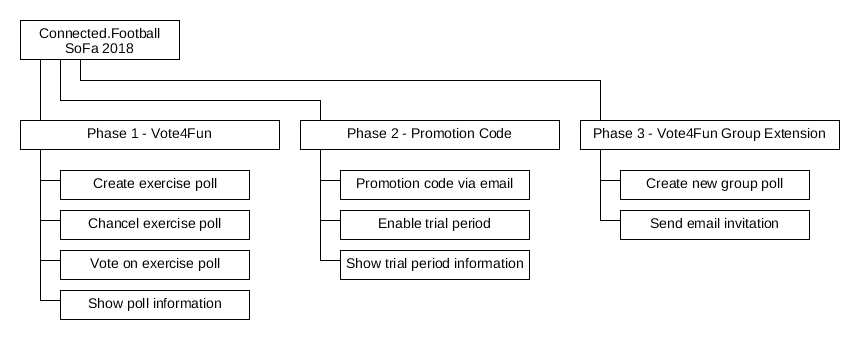
\includegraphics[width=\textwidth]{images/wbs.png}
	\caption{Work Breakdown Structure}
\end{figure}
\subsubsection{Validate Scope}
As this project progresses the team will verify interim project deliverables against the original scope. To ensure that project work remains within the scope of the project those interim deliverables will be discussed in weekly meetings with the product owner.
\subsubsection{Control Scope}
The project team will work together to control of the scope of the project. The project manager will oversee the project team and the progression of the project to ensure that this scope control process if followed.\\
If a change to the project scope is needed, all team members and the product owner must approve of the scope change.

%%%%%%%%%%%%%%%%%%%%%%%%%%%%%%%%%%%%%%%%%%%%%%%%%%
%% TIME MANAGEMENT
%%%%%%%%%%%%%%%%%%%%%%%%%%%%%%%%%%%%%%%%%%%%%%%%%%

\subsection{Time Management}
\label{ssec:time_management}

TODO Patrick


%%%%%%%%%%%%%%%%%%%%%%%%%%%%%%%%%%%%%%%%%%%%%%%%%%
%% COST MANAGEMENT
%%%%%%%%%%%%%%%%%%%%%%%%%%%%%%%%%%%%%%%%%%%%%%%%%%

\subsection{Cost Management}
\label{ssec:cost_management}

This subsection deals with the cost management of the project in question. It is being detailed how cost were managed in the project and how costs and expenses were monitored over the course of the project.
\newline
Costs did not play a vital role in the project. Given that the project is part of a University module, the project team is working without compensation and all resources, such as they are mentioned in \textit{Subsection \ref{ssec:procurement_management}}, are being provided by the client.
\newline
Cost management was considered during the project planning due to the small likelihood that the project requires further resources. In this case, the responsibility for providing these resources were that of the client. However, the project team would have been responsible for defining why the new resource is necessary for development and on what scale the resource needs to be provided. However, such a case never occurred during the course of the project is only mentioned for the purpose of completeness.


%%%%%%%%%%%%%%%%%%%%%%%%%%%%%%%%%%%%%%%%%%%%%%%%%%
%% STAKEHOLDER MANAGEMENT
%%%%%%%%%%%%%%%%%%%%%%%%%%%%%%%%%%%%%%%%%%%%%%%%%%

\subsection{Stakeholder Management}
\label{ssec:stakeholder_management}

TODO Lucas


%%%%%%%%%%%%%%%%%%%%%%%%%%%%%%%%%%%%%%%%%%%%%%%%%%
%% HUMAN RESOURCE MANAGEMENT MANAGEMENT
%%%%%%%%%%%%%%%%%%%%%%%%%%%%%%%%%%%%%%%%%%%%%%%%%%

\subsection{Human Resource Management}
\label{ssec:human_resource_management}

TODO Patrick


%%%%%%%%%%%%%%%%%%%%%%%%%%%%%%%%%%%%%%%%%%%%%%%%%%
%% COMMUNICATION MANAGEMENT
%%%%%%%%%%%%%%%%%%%%%%%%%%%%%%%%%%%%%%%%%%%%%%%%%%

\subsection{Communication Management}
\label{ssec:communication_management}

TODO Lucas


%%%%%%%%%%%%%%%%%%%%%%%%%%%%%%%%%%%%%%%%%%%%%%%%%%
%% RISK MANAGEMENT
%%%%%%%%%%%%%%%%%%%%%%%%%%%%%%%%%%%%%%%%%%%%%%%%%%

\subsection{Risk Management}
\label{ssec:risk_management}

TODO Patrick


%%%%%%%%%%%%%%%%%%%%%%%%%%%%%%%%%%%%%%%%%%%%%%%%%%
%% PROCUREMENT MANAGEMENT
%%%%%%%%%%%%%%%%%%%%%%%%%%%%%%%%%%%%%%%%%%%%%%%%%%

\subsection{Procurement Management}
\label{ssec:procurement_management}

Part of the Project Management process is to manage the processes necessary to acquire services and products that ensure the ability to work on the project. This includes both management services as well as external software products used in development.
\newline
The project encompassed the following products and services. It is detailed how they were used in the project and who was responsible for providing them.

\subsubsection{Atlassian \textit{Jira}}
\label{sssec:jira}

\begin{figure}[H]
    \begin{center}
        
\includegraphics[width=0.3\textwidth]{images/logos/jira-logo.png}
        \caption{Atlassian \textit{Jira} Logo}
        \label{fig:jira_logo}
    \end{center}
\end{figure}

To manage the agile process of the project, \textit{Jira} by Atlassian was made use of. The platform allowed the project team members to keep track of the backlog of tasks and user stories and to manage them in Scrum sprints.
\newline
\textit{Jira} was provided by the client \textit{Connected.Football}. The client was responsible for granting the other team members and stakeholders access to the tool and to ensure that certain team members have the necessary permissions to interact with the provided tool set. The developing team members were responsible for keeping the content of the created \textit{Jira} boards correct and up-to-date.

\subsubsection{\textit{GitHub}}
\label{sssec:github}

\begin{figure}[H]
    \begin{center}
        
\includegraphics[width=0.2\textwidth]{images/logos/github-logo.png}
        \caption{\textit{GitHub} Logo}
        \label{fig:github_logo}
    \end{center}
\end{figure}

The developed \textit{React Native} product was being versioned using \textit{Git}, which uses \textit{GitHub} as a platform. The client was again responsible for providing the team members access to the versioning system and to ensure that the provided sources are in a state that enables development by the project team.
\newline
The project team was responsible for committing changes they make to the product to the \textit{GitHub} repository, including accurate descriptions of what has been changed since the last commit. It was also the responsibility of the team to resolve commit errors and conflicts, as well as to minimise the likelihood of such occurrences.

\subsubsection{\textit{Subversion}}
\label{sssec:subversion}

Another versioning system used over the course of the project was \textit{Subversion}. This system was used to commit and share University-related artefacts and documents, such as this project report.
\newline
Fontys Hogeschool Techniek en Logistiek Venlo was responsible for the availability and integrity of the repositories in question. Again, it was the responsibility of the team members to ensure a working state of the repositories and to commit changes with accurate descriptions.

\subsubsection{\textit{Firebase}}
\label{sssec:firebase}

\begin{figure}[H]
    \begin{center}
        
\includegraphics[width=0.2\textwidth]{images/logos/firebase-logo.png}
        \caption{\textit{Firebase} Logo}
        \label{fig:firebase_logo}
    \end{center}
\end{figure}

Some backend functionality of the product was relying on Google's \textit{Firebase}. It was for example used to send push notifications to mobile user devices.
\newline
It was the responsibility of the client to ensure that the project team has the necessary rights to interact with the already set up \textit{Firebase} backend. On the other hand, the team was responsible for interacting with the backend in a proper way, ensuring the integrity of the provided data and infrastructure. The project team did not have any access to the backend in the sense of interacting with the interface provided by Google, but by using it by referencing and using it in the source code of the application.

\subsubsection{Integrated development environments}
\label{sssec:ides}

\begin{figure}[H]
    \begin{center}
        
\includegraphics[width=0.2\textwidth]{images/logos/visual-studio-code-logo.png}
        \caption{\textit{Visual Studio Code} Logo}
        \label{fig:visual-studio-code_logo}
    \end{center}
\end{figure}

The project team used some integrated development environments (IDEs) to develop the product, most notably \textit{Visual Studio Code}. The IDE was used to inspect and change the source code of the product.
\newline
The developer was responsible for the functionality of the IDE. The team was able to use the IDEs as they are all provided through open source. It was their responsibility to use the IDE as intended and to figure out how to resolve errors in the event that they occur. No such errors occurred during the course of the project.

\subsubsection{\textit{Node.js} Modules}
\label{sssec:nodejs_modules}

\begin{figure}[H]
    \begin{center}
        
\includegraphics[width=0.3\textwidth]{images/logos/node-js-logo.png}
        \caption{\textit{Node.js} Logo}
        \label{fig:node-js-logo}
    \end{center}
\end{figure}

The product used various \textit{Node.js} modules to offer functionality in the product. These modules were available from various repositories.
\newline
The developers of the \textit{Node.js} modules were responsible for the development of the \textit{Node.js} modules themselves and for the documentation that comes with them. Since the modules were published as open source, the project team is responsible for handling errors that occurred during the development involving their usage. They were furthermore responsible for implementing the usage of the modules in the product as the developer intended and documented.
\newline
Some of the \textit{Node.js} modules were developed by the client. Their integrity was therefore their responsibility.

\subsubsection{\textit{Slack}}
\label{sssec:slack}

\begin{figure}[H]
    \begin{center}
        
\includegraphics[width=0.2\textwidth]{images/logos/slack-logo.png}
        \caption{\textit{Slack} Logo}
        \label{fig:slack-logo}
    \end{center}
\end{figure}

The development team used \textit{Slack} to communicate outside of personal meetings, both in communication with each other as well as with the client. It was also used to share information, such as documents and source code snippets, in a non-persistent way. Configuration files that were not supposed to be uploaded to \textit{GitHub} were also shared using \textit{Slack}.
\newline
The availability of the application was ensured by the developer. It was the responsibility of the client to enable that the development team is able to join and use the \textit{Slack} platform. The project team had the responsibility to not share any sensitive information, such as credentials, over this platform.

%% ANALYSIS
\section{Analysis}
\label{sec:analysis}
\lhead{\thesection \space Analysis}

This chapter describes how the project's requirements and the customer's expectations are broken down in specific activities to reflect the behaviour of the software.
First all use cases are collected. Then the use cases are assigned to specific epics - a logical collection of use cases. Afterwards the resulting Software Requirement Specification for the first epic is presented. Finally a brief overview of the application architecture is given.

\subsubsection{Use Case Diagram}
\label{sssec:use_case_diagram}

The Use Case Diagram allows a quick overview of the main features the application has. It describes the activities that should be accessible to the different stakeholders.\\

\begin{figure}[H]
    \begin{center}
        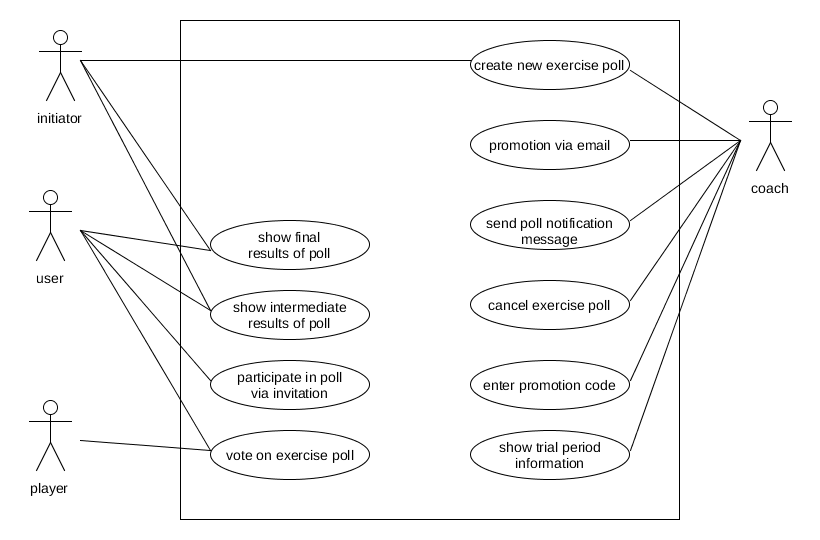
\includegraphics[width=\textwidth]{images/ucd.png}
        \caption{Use Case Diagram}
        \label{fig:ucd}
    \end{center}
\end{figure}

\subsection{Epics}
\label{ssec:epics}

To break down the development every use cases is assigned to a specific epic. An epic contains of use cases that have similar dependencies or depend on one another.

\subsubsection{Epic 1 - Vote4Fun}
\label{sssec:epic1}

The first epic includes the use cases needed to have a voting system for already registered users. They are allowed to vote on an exercise based on team membership and the coaches invitations of users by e-mail address.

The use cases relevant to the first epic are the following:

\begin{itemize}
    \item UC – 1.1 
    \newline
    Create new exercise poll.
    \item UC – 1.2 
    \newline
    Cancel exercise poll.
    \item UC – 1.3 
    \newline
    Vote on exercise poll.
    \item UC – 1.4 
    \newline
    Show final result of exercise poll.
    \item UC – 1.5 
    \newline
    Show intermediate result of exercise poll.
\end{itemize}

\subsubsection{Epic 2 - Promotion Code}
\label{sssec:epic2}
In addition to Epic 1, a coach user should be able to use a trial promotion code if he / she doesn't have the regular "\textit{VOTE4FUN}" feature to manage and start a \textit{Vote4Fun} poll for his / her team. 
\newline
This trial includes (a combination of):
\begin{itemize}
    \item A trial period in days
    \item A  maximum number of  voting polls to be created and managed
\end{itemize}
The period and number of polls for each trial code should be flexible. 
\newline
The trial code can be received via email with a \textit{promotion link, promotion code (string of characters)} or as a \textit{notification} on his /  her phone. 
\newline
\newline
The following requirements were given for this epic:
\begin{itemize}
    \item UR – 2.1 
    \newline
    A coach can open a view (position to be determined) to enter a trial code for managing Vote4Fun polls if and only if the user does not have the Vote4Fun permission.
    \item UR – 2.2
    \newline
    A coach can enter and submit a trial code.
    \item UR – 2.3 
    \newline
    A user receives a confirmation after entering the trial code.
    \item UR – 2.4 
    \newline
    A user receives a positive confirmation after entering a valid trial code.
    \item UR – 2.5 
    \newline
    A user receives a negative confirmation after entering an invalid trial code.
    \item UR – 2.6
    \newline
    A user can create and manage Vote4Fun polls after entering a valid trial code.
    \item UR – 2.7 
    \newline
    A user can see the remaining trial period / number of polls to be managed.
    \item UR – 2.8
    \newline
    A user with the app installed can click on an email promotion link to have the promotion code entered automatically.
    \item UR – 2.9 
    \newline
    A user with the app installed can click on a notification to have the promotion code entered automatically.
\end{itemize}

\subsubsection{Epic 3 - TODO Add Name}
\label{sssec:epic3}

TODO Patrick

\subsection{Application Architecture}
\label{ssec:application_architecture}

\begin{figure}[H]
    \begin{center}
        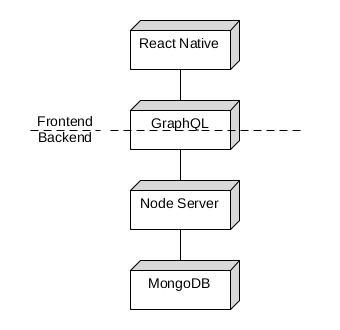
\includegraphics[width=\textwidth/2]{images/overview.png}
        \caption{Architecture Overview}
        \label{fig:architecture_overview}
    \end{center}
\end{figure}

The applications' frontend is based on \textit{React Native}, it uses \textit{GraphQL} to communicate with a node server saving its data in a \textit{MongoDB} database.

\subsection{Software Requirements Specification}
\label{ssec:software_requirements_specification}

TODO Marco

%% DESIGN
\section{Design}
\label{sec:desgin}
\lhead{\thesection \space Design}

TODO Lucas

\subsection{Functionality}
\label{ssec:functionality}

Since the application is supposed to offer a certain set of features to the user, it needed to be defined what kind of functionality was necessary to ensure that a user could interact with all the features the application has to offer. This section details this set of features and their functionality.
\newline
Each functionality is described using a set of diagrams, such as state machine or activity diagrams. A visual representation can also be found in \textit{\ref{ssec:visual_design} \nameref{ssec:visual_design}}.

\subsubsection{Creating a new Poll}
\label{sssec:creating_a_new_poll}

Since the \textit{Vote4Fun} extension is about creating a poll and letting users vote on it, the actual creation of such a poll is of course an important and arguably biggest piece of functionality. The polls are divided into two categories, which are a regular and an "on-the-fly" poll.
\newline
The regular poll is created for one specific team, as shown in Figure \ref{fig:state_machine_diagram_create_poll}. The owner of the poll simply picks a team and is able to add guests to the poll afterwards. Each guest is checked for validity, in this case whether the entered email address representing the guest is an active user of \textit{Connected.Football}. This can be repeated for multiple users. An "on-the-fly" poll does not require a team, but rather a set of email addresses, which do not need to be registered on \textit{Connected.Football}. Once the owner has entered the email addresses, a temporary team is created (see \textit{\ref{sssec:creating_temp_team} \nameref{sssec:creating_temp_team}}).
\newline
In both cases, the poll has a set of users. Once the owner enters information regarding the deadline and exercises to be voted upon, the poll itself is created. This is followed by notifications being sent to all users participating in the poll.

\begin{figure}[H]
    \begin{center}
        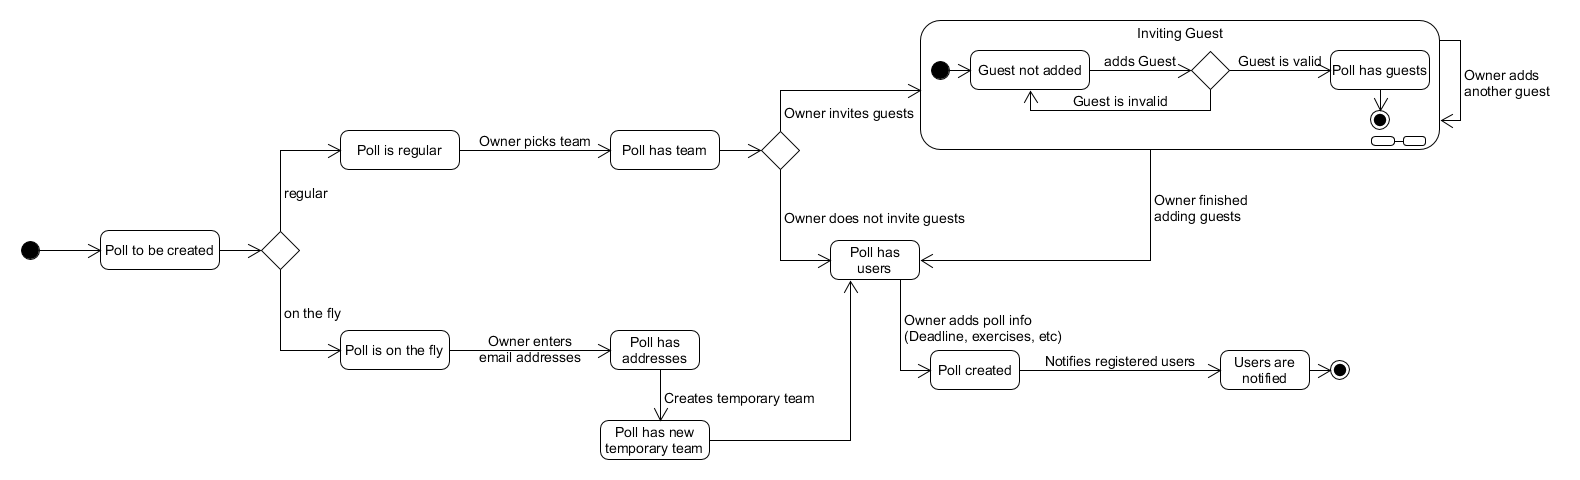
\includegraphics[width=1\textwidth]{images/diagrams/state_machine_diagrams/StateDiagram_CreatePoll.png}
        \caption{State Machine Diagram Create Poll}
        \label{fig:state_machine_diagram_create_poll}
    \end{center}
\end{figure}

TODO Lucas Describe Activity Diagram Create Exercise Poll

\begin{figure}[H]
    \begin{center}
        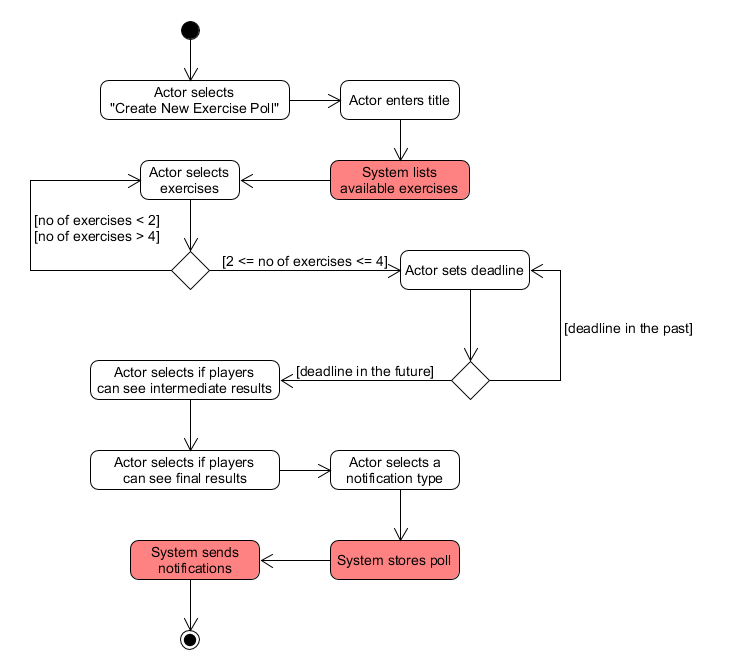
\includegraphics[width=0.8\textwidth]{images/diagrams/activity_diagrams/ActivityDiagram_CreateExercisePoll.png}
        \caption{Activity Diagram Create Poll}
        \label{fig:activity_diagram_create_poll}
    \end{center}
\end{figure}

\subsubsection{Creating a Temporary Team}
\label{sssec:creating_temp_team}

As mentioned in \textit{\ref{sssec:creating_a_new_poll} \nameref{sssec:creating_a_new_poll}}, when an "on-the-fly" poll is created, a new temporary team is created as well. This team consists of people that may or may not be registered with the \textit{Connected.Football} platform. Unfortunately, this functionality was not implemented in time, but since it is required for Epic 3 (see \textit{\ref{sssec:epic3} \nameref{sssec:epic3}}, it is mentioned for the sake of completeness and for future reference.
\newline
As seen in Figure \ref{fig:state_machine_diagram_create_temp_team}, the process starts with the owner of the poll entering an email address representing the person they want to add to the temporary team. If the email is not properly formatted, the entry is discarded. If the format is correct, the address is stored and the owner can either add another email address or they can continue.
\newline
The \textit{Connected.Football} platform than checks for every entered email address whether a user with the same address is already registered. If that is the case, the reference to the already existing user is stored in the temporary team and the user is sent a push notification. If not, the platform creates a callback and sends an invitation to the email address. This invitation was supposed to be handled by \textit{Firebase}, which provides functionality for such an on-boarding process. If the user follows this invitation, the callback is triggered, which stores the new user in the temporary team, once they have completed their registration.

\begin{figure}[H]
    \begin{center}
        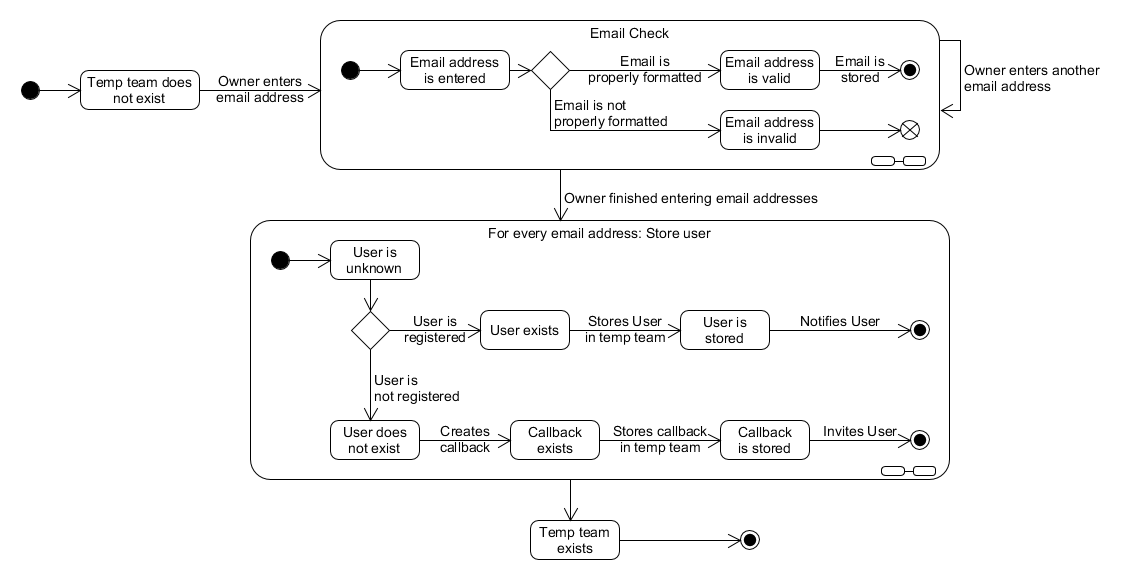
\includegraphics[width=1\textwidth]{images/diagrams/state_machine_diagrams/StateDiagram_CreateTempTeam.png}
        \caption{State Machine Diagram Create Temporary Team}
        \label{fig:state_machine_diagram_create_temp_team}
    \end{center}
\end{figure}

\subsubsection{Voting on an Exercise Poll}
\label{sssec:voting_on_exercise_poll}

TODO Lucas Describe Activity Diagram Vote on Poll

\begin{figure}[H]
    \begin{center}
        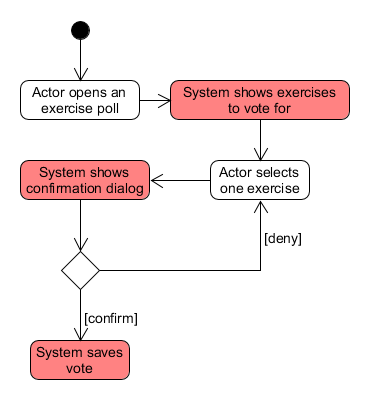
\includegraphics[width=0.5\textwidth]{images/diagrams/activity_diagrams/ActivityDiagram_VoteOnExercisePoll.png}
        \caption{Activity Diagram Vote on Poll}
        \label{fig:activity_diagram_vote_on_poll}
    \end{center}
\end{figure}

\subsubsection{Entering a Promotion Code}
\label{sssec:entering_promotion_code}

TODO Lucas Describe Activity Diagram Enter Promotion Code

\begin{figure}[H]
    \begin{center}
        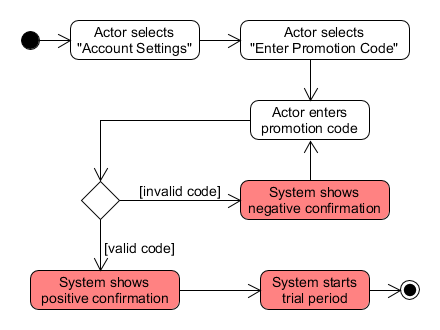
\includegraphics[width=0.6\textwidth]{images/diagrams/activity_diagrams/ActivityDiagram_EnterPromotionCode.png}
        \caption{Activity Diagram Enter Promotion Code}
        \label{fig:activity_diagram_enter_promotion_code}
    \end{center}
\end{figure}

\subsection{Visual Design}
\label{ssec:visual_design}

TODO Lucas, TODO Marco

\subsection{\textit{Vote4Fun} Object Definition}
\label{ssec:vote4fun_object_definition}

TODO Marco

\subsection{Component Structure}
\label{ssec:component_structure}

Given the component-based structure of the \textit{React Native} framework, some new components had to be designed to implement the necessary functionality of the \textit{Vote4Fun} extension. This section details how the Setup Wizard, which is the main part of the extension, was designed, specifically how it's components are placed in relation to each other and to the existing \textit{Connected.Football} application.

\begin{figure}[H]
    \begin{center}
        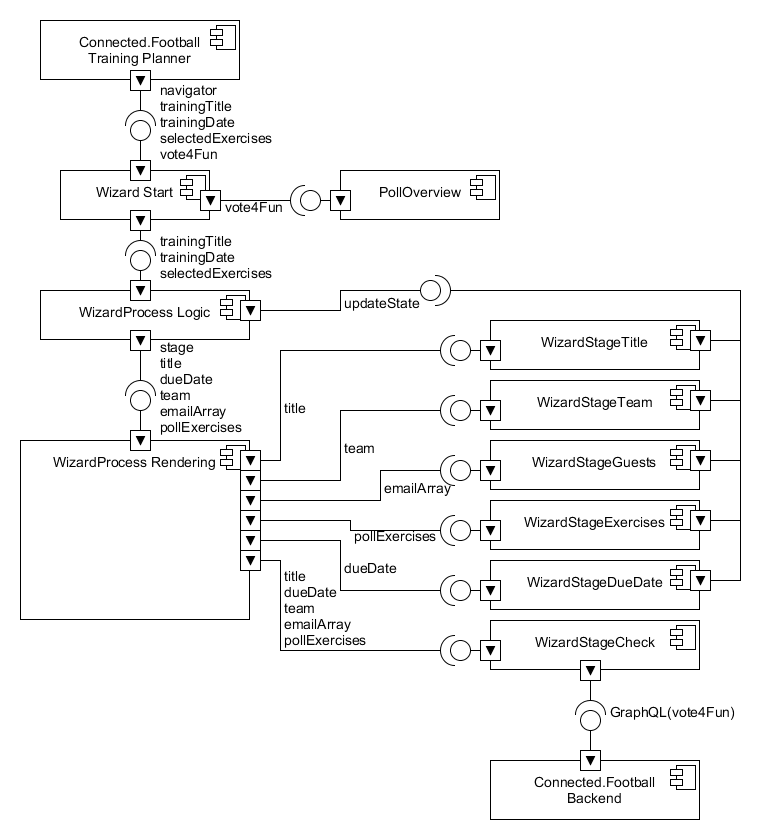
\includegraphics[width=0.9\textwidth]{images/diagrams/component_diagrams/ComponentDiagram_Wizard.png}
        \caption{Component Diagram Poll Setup Wizard}
        \label{fig:component_diagram_wizard}
    \end{center}
\end{figure}

Figure \ref{fig:component_diagram_wizard} shows a component diagram containing all the major components involved in the poll Setup Wizard. The Wizard itself is being used by the \textit{Connected.Football Training Planner}. This was done as a poll is intrinsically linked to a training program and is dependent on one.
\newline
The Wizard itself has an overarching component called \textit{WizardStart}. This is a component that is shown as part of the training planner, displaying either a simple start button to start the setup or an overview in form of the component \textit{PollOverview}, if a \textit{vote4Fun} object is supplied by the training planner. In any case, the component is also supplied with the state of \textit{trainingTitle}, \textit{trainingDate} and \textit{selectedExercises}, as well as a reference to the \textit{navigation} component, since the \textit{WizardProcess} component is called as a new element on the navigation stack of the application.
\newline
The \textit{WizardProcess} is divided into two parts, namely \textit{WizardProcess Logic} and \textit{WizardProcess Rendering}. These are actually parts of the same file, which is a functional component making use of \textit{recompose}. For further information about functional components, see \textit{\ref{ssec:recompose} \nameref{ssec:recompose}}.
\newline
\textit{WizardProcess Logic} handles the business logic and supplies \textit{WizardProcess Rendering} with a state for \textit{stage}, \textit{title}, \textit{dueDate}, \textit{team}, \textit{emailArray} and \textit{pollExercises}. Depending on the value of \textit{stage}, \textit{WizardProcess Rendering} than renders one of the components \textit{WizardStageTitle}, \textit{WizardStageTeam}, \textit{WizardStageGuests}, \textit{WizardStageExercises}, \textit{WizardStageDueDate} and \textit{WizardStageCheck}, in that order.
\newline
Each of the \textit{WizardStage} components is responsible for taking a user's input and sending it to the \textit{WizardProcess Logic} component using a callback function. The \textit{WizardProcess Logic} checks if the user input is valid, which includes the usage of the properties supplied to it by the \textit{WizardStart} component, and sets the state to the user input if it is deemed valid.
\newline
Finally, the \textit{WizardStageCheck} component received all the entered values as properties to render them one last time for the user to check their input. Afterwards, the component triggers a call to the \textit{Connected.Football} backend server, sending a \textit{GraphQL} mutation, which creates a new \textit{Vote4Fun} object on the backend and takes other necessary actions, such as notifying users.
\newline
Aside from the components mentioned above, most components make use of simpler components, such as text entry fields or buttons. These are already supplied by \textit{React Native} or other packages that were loaded. Some custom components were defined over the course of this project, however, they only defined simple logic and rendering and are therefore not mentioned in detail here.

%% IMPLEMENTATION
\section{Implementation}
\label{sec:implementation}
\lhead{\thesection \space Implementation}

This chapter details how the \textit{Vote4Fun} extension was implemented over the course of the project, based on the design described in \textit{\ref{sec:desgin} \nameref{sec:desgin}}. To do so, the implementation of the Setup Wizard is explained first. Given the component-based structure of \textit{React Native}, each component that makes up the Setup Wizard is explained, as they are defined in Figure \ref{fig:component_diagram_wizard} in \textit{\ref{ssec:component_structure} \nameref{ssec:component_structure}}. Each component section contains a simplified version of it's source code to highlight important points about their implementation. The entire structure of the Wizard is described too, as well as how each child component interacts with it using callback functions.
\newline
The description of the individual components is followed by a definition of functional components, as well as how they were used during the project in combination with \textit{recompose}. It is detailed how to write functional components and why it is a good idea to use them. This section also includes an overview and description of the functionality of \textit{recompose} that was used in the extension.
\newline
What follows is a description of how \textit{GraphQL} was used during the project. It briefly details what \textit{GraphQL} is and what makes it great to use. This is followed by an explanation of how it was implemented in the application and where it was used as part of the extension.
\newline
The chapter closes with a section about the problems occurring during development. The problems described deal with the way \textit{React Native} applications can be debugged and why that way is less efficient than it could be as well as problems occurring because of \textit{Node.js} packages being used, including a way to fix most problems related to this issue. It is also detailed how configuration errors took place during the implementation, specifically how the application failed to be deployed to an \textit{iOS} device.

\subsection{Poll Wizard}
\label{ssec:poll_wizard}

The Poll Wizard is mostly defined by the \textit{WizardProcess} component. A simplified version of this component can be seen in Listing \ref{lst:wizardComponentWithRecompose}. All source code that does not relate to the staging functionality of the Wizard was removed from the code below.

\begin{lstlisting}[language=javascript,caption=Simplified Wizard Component using \textit{recompose},label=lst:wizardComponentWithRecompose]
const WizardProcess = ({stage, incrementStage, decrementStage}) => {
  return (
    <View>
      {stage == 0 && <WizardStageTitle />}
      {stage == 1 && <WizardStageTeam />}
      {stage == 2 && <WizardStageGuests />}
      {stage == 3 && <WizardStageExercises />}
      {stage == 4 && <WizardStageDueDate />}
      {stage == 5 && <WizardStageCheck />}

      <View>
        {stage != 0 && (
          <TouchableOpacity onPress={decrementStage}>
            <Icon name='arrow-circle-left' size={60} />
          </TouchableOpacity>
        )}
        {(stage >= 0 && stage <= 4) &&
          <TouchableOpacity onPress={incrementStage}>
            <Icon name='arrow-circle-right' size={60} />
          </TouchableOpacity>
        }
        {stage == 5 && (
          <TouchableOpacity onPress={buildVote4FunObject}>
            <Icon name='check-circle' size={60} />
          </TouchableOpacity>
        )}
      </View>
    </View>
  )
}
export default compose(
  withState('stage', 'setStage', 0),
  withHandlers({
    incrementStage: props => () => {props.setStage(props.stage + 1)},
    decrementStage: props => () => {props.setStage(props.stage - 1)},
  mapProps(props => ({
    stage: props.stage,
    incrementStage: props.incrementStage,
    decrementStage: props.decrementStage,
  }))
)(WizardProcess)
\end{lstlisting}

The component is actually divided into two components, making use of \textit{recompose}. For further information about \textit{recompose}, see \textit{\ref{ssec:recompose} \nameref{ssec:recompose}}. The first part is a functional component, which takes a numerical value for \textit{stage} as well as functions to change this value as parameters. Depending on the value of \textit{stage}, different components are rendered, as described in \textit{\ref{ssec:component_structure} \nameref{ssec:component_structure}}. The component furthermore renders buttons depending on certain \textit{stage} values, to advance through the stages of the Setup Wizard. The complete component also implements certain checks at this point, for example by only showing the advancing button when a title has been entered in the \textit{WizardStageTitle} component.
\newline
The second part of the component defines the business logic of the component. It uses \textit{recompose} to provide state, in this example to the property \textit{stage}. The full component defines the entire state of all mutable values here, including the handlers to change them. These handlers are used as callback methods by the \textit{WizardStage} components to store entered values. All values and functions created this way are also mapped as properties, so that they can be used by the functional rendering component.
\newline
Since the component strictly separates rendering and logic, the component can easily be expanded. More stages could potentially be added or removed. Given the right handlers, stages could also be skipped or jumped to.

\subsubsection{Poll Title}
\label{sssec:poll_title}

The \textit{WizardStageTitle} component, as it is seen in Listing \ref{lst:pollTitleComponent}, is a fairly simple one. It shows a text input field for the user to put in the name of the poll. Just like \textit{WizardProcess}, it is a functional component, albeit without \textit{recompose}.

\begin{lstlisting}[language=javascript,caption=Simplified Poll Title Component,label=lst:pollTitleComponent]
const WizardStageTitle = (props) => {
  if (props.title.length == 0) {
    props.updateTitle("Poll: " + props.trainingTitle)
  }
  return (
    <View style={props.styles.stageContainer}>
      <Text style={props.styles.header}>
        {I18n.t('SOFA_wizard_header_title')}
      </Text>
      <FormTextInput
        value={props.title}
        label=''
        maxLength={50}
        placeholder={`${I18n.t('SOFA_wizard_title_placeholder')}`}
        onChangeText={props.updateTitle} />
    </View>
  );
};
export default WizardStageTitle;
\end{lstlisting}

If the component is initialised the first time, still having an empty string as a value for \textit{title}, which is given to the component as a property, the component gives it a default value, consisting of the value "Poll: " and the original training title, which is also a property. In \textit{\ref{ssec:component_structure} \nameref{ssec:component_structure}} you can see that the training title is in turn provided as a property to the \textit{WizardProcess} component.
\newline
Other than that, the component makes use of the \textit{FormTextInput}, which is a custom styled text entry field component. The callback function is referenced in the "onChangeText" property. Furthermore, the component is referencing the \textit{I18n} component, which can load specified strings for different languages, making it easy to translate the application into different languages and changing them as needed. The style of the components is also loaded as property, since \textit{WizardProcess} defines most styles to keep the style consistent throughout all \textit{WizardStage} components.

\subsubsection{Team Selection}
\label{sssec:poll_team}

TODO Patrick

\subsubsection{Addition of Guests}
\label{sssec:poll_guests}

The \textit{WizardStageGuests} component allows the user to invite guests via email to participate in the voting for the exercise for a specific training. One condition for this is that the email that is invite to the poll is already registered in the \textit{Connected.Football} environment. 
\newline
The structure of the component in Listing \ref{lst:pollGuestsComponent} is fairly simple. It has a text input where the user can enter an email and a button that will then check this email and when the check returns true, it will add the email to a \textit{FlatList}. 
\begin{lstlisting}[language=javascript, caption=Simplified Guest Component, label=lst:pollGuestsComponent]
return (
    <ApolloConsumer>
      {client => ...
        }
        return (
          <View>
            <View style={props.styles.stageContainer}>
              <Text style={props.styles.header}>
                {I18n.t('SOFA_wizard_header_guests')}
              </Text>
              <FormTextInput
                value={props.email}
                label={`${I18n.t('SOFA_wizard_guests_email')}`}
                maxLength={50}
                type='email-address'
                placeholder={`${I18n.t('SOFA_wizard_guests_enter_email')}`}
                onChangeText={props.updateEmail}
              />
              <Button
                title={`${I18n.t('SOFA_wizard_guests_add_button')}`}
                color='green'
                onPress={onPress}
              />
            </View>
            <FlatList
              data={props.emailArray}
              extraData={props.updateView}
              renderItem={({ item }) => (
              ...
              )}
              keyExtractor={(item, index) => index.toString()}
            />
          </View>
        )
      }}
    </ApolloConsumer>
  )
}
\end{lstlisting}

In Listing \ref{lst:pollGuestsCheck} the methods that check the email on the offline part (no connection to the \textit{Connected.Football} environment) are shown. The method \textit{validateEmail} gets an email as a parameter and then checks the email if the email has the standard email format. The second method checks if the email is already in the \textit{emailArray}. This way the \textit{FlatList} can't have the same email twice.

\begin{lstlisting}[language=javascript, caption=Check E-Mail Methods, label=lst:pollGuestsCheck]
const validateEmail = email => {
  var re = /^(([^<>()\[\]\\.,;:\s@"]+(\.[^<>()\[\]\\.,;:\s@"]+)*)|(".+"))@((\[[0-9]{1,3}
    \.[0-9]{1,3}\.[0-9]{1,3}\.[0-9]{1,3}])|(([a-zA-Z\-0-9]+\.)+[a-zA-Z]{2,}))$/
  return re.test(email)
}
const isDoubleEmail = (value, array) => {
  const bufArray = array
  let doubleEmail = false
  bufArray.find(item => {
    if (item.email === value) {
      doubleEmail = true
    }
  })
  return doubleEmail
}
\end{lstlisting}

\subsubsection{Choice of Exercises}
\label{sssec:poll_exercises}

TODO Marco

\subsubsection{Due Date Settings}
\label{sssec:poll_due_date}

The component that takes user input regarding the due date of a poll, which is called \textit{WizardStageDueDate}, as seen in Listing \ref{lst:pollDueDateComponent}, is very similar to the component mentioned in \textit{\ref{sssec:poll_title} \nameref{sssec:poll_title}}. It is again a simple functional component which receives relevant values as properties to render the user input field.

\begin{lstlisting}[language=javascript,caption=Simplified Poll Due Date Component,label=lst:pollDueDateComponent]
const WizardStageDueDate = (props) => {
  return (
    <View style={props.styles.stageContainer}>
      <Text style={props.styles.header}>
        {I18n.t('SOFA_wizard_header_due_date')}
      </Text>
      <DateTimePicker
        label="SOFA_wizard_due_date"
        trainingDate={props.dueDate}
        setTrainingDate={props.updateDueDate}
      />
      <View style={styles.hintContainer}>
        <Text style={styles.hintText}>
          {I18n.t('SOFA_wizard_due_date_hint')}
        </Text>
      </View>
    </View>
  );
};
export default WizardStageDueDate;
\end{lstlisting}

The component makes use of another component called \textit{DateTimePicker}, which is a custom component that opens a dialog which is native to the mobile OS the application was deployed to, which lets the user pick a date and time. Once a user has chosen a time, the component calls the supplied callback function, in this case "updateDueDate".
\newline
Given the nature of a poll, this due date of course has to be before the date of the actual training. Such a check is absent in the component mentioned above. The actual check is done by the \textit{WizardProcess} component, which handles most of the logic.

\begin{lstlisting}[language=javascript,caption=Increment Stage Check,label=lst:incrementStageCheck]
{((stage == 0 && title != '') ||
   stage == 1 ||
   stage == 2 ||
   stage == 3 ||
   ((stage == 4) && (dueDate > new Date().addDays(1)) && (dueDate.addHours(2) < trainingDate))
) &&
  <TouchableOpacity onPress={incrementStage}>
    <Icon name='arrow-circle-right' size={60} />
  </TouchableOpacity>
}
\end{lstlisting}

The source code listed in Listing \ref{lst:incrementStageCheck} shows the check as to whether to show the button which advances the Setup Wizard to it's next stage. The button is only rendered when certain conditions are met, for instance, in stage 0, which makes use of the component \textit{WizardStageTitle}, the title itself must not be empty. In the same way, the entered due date must be at least one day in the future, so that users have time to vote, and at least two hours before the start of the training.
\newline
As far as state is concerned, the component acts the same way as \textit{WizardStageTitle}. Once the callback function is called, the state is stored into the variable "dueDate" and is available to be used in the entire Setup Wizard components and it's sub-components.

\subsubsection{Check of Settings}
\label{sssec:poll_check}

TODO Marco Check and proof-read section, add information as you see fit 

Listing \ref{lst:pollCheckComponent} shows a simplified version of the \textit{WizardStageCheck} component. Again a functional component, the component seems to include quite a lot, yet it is actually only responsible for showing the already entered values to the user. The amount of source code simply comes from the amount of information that needs to be displayed, which includes information from all previous \textit{WizardStage} components.

\begin{lstlisting}[language=javascript,caption=Simplified Poll Check Component,label=lst:pollCheckComponent]
const WizardStageCheck = (props) => {
  return (
    <View>
      <Text>{I18n.t('SOFA_wizard_header_check')}</Text>
      <View>
        <FormLabel>{I18n.t('SOFA_wizard_title')}</FormLabel>
        <View>
          <Text>{props.title}</Text>
        </View>
        {props.emailArray.length > 0 &&
          <View>
            <FormLabel>{I18n.t('SOFA_wizard_guests')}</FormLabel>
            <View>
              <FlatList
                data={props.emailArray}
                renderItem={({ item }) => (
                  <View>
                    <Text>{item.email}</Text>
                  </View>
                )}
                keyExtractor={(item, index) => index.toString()}/>
            </View>
          </View>
        }
        <FormLabel>{I18n.t('SOFA_wizard_exercises')}</FormLabel>
        <View>
          <Text>{props.pollExercises}</Text>
        </View>
        <FormLabel>{I18n.t('SOFA_wizard_due_date')}</FormLabel>
        <View>
          <Icon name="date-range" size={40} />
          <Text>{moment(props.dueDate).format('DD-MM-YYYY H:mm')}</Text>
        </View>
      </View>
    </View>
  );
};
export default WizardStageCheck;
\end{lstlisting}

The component itself does not actually trigger any callback method, as the interaction for sending the checked information is actually part of the stage buttons displayed by the \textit{WizardProcess} component. Listing \ref{lst:wizardComponentWithRecompose} in \textit{\ref{ssec:poll_wizard} \nameref{ssec:poll_wizard}} contains the button which calls the handler method "buildVote4FunObject", which is responsible for sending the entered information to the \textit{Connected.Football} backend. This handler method can be seen in Listing \ref{lst:buildVote4FunObject}.

\begin{lstlisting}[language=javascript,caption=\textit{buildVote4FunObject} Handler Method,label=lst:buildVote4FunObject]
[...]
export default compose(
  //[...]
  withHandlers({
    buildVote4FunObject: props => () => {
      const exercises = [];
      props.pollExercises.forEach(function (entry) {
        exercises.push({ "exerciseId": entry.id, "playerIds": [] });
      })
      const v4l = {
        "type": "clubteam",
        "title": props.title,
        "deadline": props.dueDate,
        "showIntermediaResults": false,
        "showFinalResults": false,
        "notificationHoursBeforeDeadline": 1,
        "notificationAfterPercentageVoted": 50,
        "guestIDs": emailArray,
        "exercises": exercises
      }
      props.action({ type: 'setVote4Fun', text:v4l });
      props.navigator.pop();
    },
  }),
  //[...]
)(WizardProcess)
\end{lstlisting}

This method builds a JSON object that consists of all the information entered by the user as well as some default values that can be changed by the owner of the poll later, such as whether to show intermediate results or when to send notifications to users. One thing to pay attention to is how the "exercises" array is constructed. The array does not only consist of the IDs of exercises, like the "pollExercises" array that was constructed by the \textit{WizardStageExercises} component (see \textit{\ref{sssec:poll_exercises} \nameref{sssec:poll_exercises}}), but of objects containing both one the mentioned IDs as well as an empty array called "playerIds". This empty array is later filled with the ID of an user, whenever this user votes for this specific exercise in the poll. This way it can be tracked who already voted and which exercises got how many views.
\newline
The constructed JSON object is then propagated to the "action" property. This property is handed down from the component creating the training planner, which includes the storing of said object as well as the \textit{GraphQL} mutation to store the poll together with the entire training plan. A simplified version of this functionality can be seen in Listing \ref{lst:trainingPlannerGraphQL}.

\begin{lstlisting}[language=javascript,caption=Simplified Training Planner Component with \textit{GraphQL} Mutation,label=lst:trainingPlannerGraphQL]
const actions = {
  //[...]
  setVote4Fun: (s, action) => Object.assign({}, s, {
    vote4fun: action.text,
  }),
};
//[...]
const SAVE_PROGRAM_MUTATION = gql`
  mutation SaveProgram($payload: JSON!) {
    saveProgram(payload: $payload) {
        data
        ...ProgramListItem
      }
  }
  ${PROGRAM_LIST_FRAGMENT}
`;
//[...]
export default compose(
  //[...]
  graphql(SAVE_PROGRAM_MUTATION),
  withReducer('programState', 'action', reducer, ({ program }) => {
    return {
      id: program.id,
      //[...]
      vote4fun: program.vote4fun || [],
    };
  }),
  withHandlers({
    saveProgram: props => () => {
      props.mutate({
        variables: {
          payload: transformReducerToPayload(props.programState),
        },
        update: (store, { data: { saveProgram } }) => {
          const data = store.readQuery({ query: PROGRAMS_QUERY });
          data.getPrograms.unshift(saveProgram);
          store.writeQuery({ query: PROGRAMS_QUERY, data });
        },
      });;
    },
  ),
)(TabView);
\end{lstlisting}

The "action" that is given to the Setup Wizard is defined at the very beginning. This callback simply receives the input of the callback call and stores the text that comes with it in a variable "vote4fun". The rest shows how all entered values of a training, including the values entered in the Setup Wizard, are merged into a "reducer" which is in turn sent as a \textit{GraphQL} mutation.
\newline
The mutation itself is defined in the lines 8-15. The mutation references "SaveProgram", which is a mutation endpoint provided by the \textit{Connected.Football} backend. The sent object itself is defined with \textit{recompose}'s "withReducer", which returns all values of a training program, including the "vote4fun" value, as a JSON object. Note that if the value "vote4fun" is null, an empty array is sent instead, since a training planner does not necessarily require a poll to be created.
\newline
Finally, the handler method "saveProgram" takes this reducer and sends it to the backend. The reducer is taken as a payload for the mutation. The mutation returns the ID of the created training program, which can be used for other functionality, such as editing the training program. Since the "vote4fun" object is part of said program, it is of course also possible to edit the poll itself.

\subsection{\textit{recompose} \& Functional Components}
\label{ssec:recompose}

\textit{recompose} is a \textit{Node.js} package which is available at \url{https://www.npmjs.com/package/recompose}. It was made heavily use of during the project because of the possibility to completely divide logic and rendering inside the same component. All major components described in \textit{\ref{ssec:component_structure} \nameref{ssec:component_structure}} are functional components. An example of a functional component can be seen in Listing \ref{lst:functionalComponent}.

\begin{lstlisting}[language=javascript,caption=Functional Component Example,label=lst:functionalComponent]
const Component = prop => (
  <View>
    <ChildComponent />
  </View>
);
\end{lstlisting}

Depending on individual preference, the strict functional arrow representation may also be extended with the "return" keyword for easier readability. The one thing to notice about such a functional component is that it does not implement any form of state or state management. What makes a functional component functional is that it is supplied with some form of state, such as properties or other state-forming values, and that it returns something that is dependent on that state, in this case a \textit{React Native} rendering definition. Given that the functional component is not dependent on how the state is managed, it can be reused in any way necessary. Two or more implementations of state and state management can make use of the same functional component without ever needing to change the component itself. The only restriction is that if the same state is supplied to the component, the result is always the same, since it does not make use or references any other form of state. For this reason, functional components are also known as stateless components.
\newline
To implement any business logic, \textit{recompose} comes into play. A simple example of the usage of \textit{recompose} can be seen in Listing \ref{lst:wizardComponentWithRecompose} in \textit{\ref{ssec:poll_wizard} \nameref{ssec:poll_wizard}}. The component defined there contains a functional component called \textit{WizardProcess} which is supplied with the properties \textit{stage}, \textit{incrementStage} and \textit{decrementStage}, which make up the state and the state management. Assuming that these properties do not change, the returned \textit{React Native} rendering always acts the exact same way.
\newline
Table \ref{tab:recomposeFunctions} shows the basic functionality and keywords of \textit{recompose}. The following description explains how to use the mentioned keywords and how they were implemented in the project.

\begin{table}[H]
    \centering
    \begin{tabularx}{\textwidth}{ |l|X| }
        \hline
        \rowcolor[HTML]{C0C0C0} 
        \textbf{Name}              & \textbf{Usage}                                                                                                                  \\ \hline
        \textit{withState}         & Manages a single state value, providing a function to update the value and accepting an optional default value.                 \\ \hline
        \textit{withHandlers}      & Creates handler methods, which are functions that do things in response to events being triggered, accepting component's props. \\ \hline
        \textit{mapProps}          & Replaces the current props with properties given inside the function.                                                           \\ \hline
        \textit{withProps}         & Merges the current props with properties given inside the function.                                                             \\ \hline
        \textit{onlyUpdateForKeys} & Limits the re-rendering of the component to changes in state defined inside the function.                                       \\ \hline
    \end{tabularx}
    \caption{\textit{recompose} Functions}
    \label{tab:recomposeFunctions}
\end{table}

The actual definition of these properties is handled by using \textit{recompose}. Making use of the "compose" command, various state and logic definitions can be supplied to the functional component, which is references in brackets at the very end. Using the "withState" keyword, the state, which is as aforementioned absent from the functional component, can be defined. Each state has a name, a name for a method which can overwrite the value of the state and default value. In the example that is "stage", "setStage" and 0, respectively. This state is initialised whenever the component using \textit{recompose} is used in another component.
\newline
Stage management and business logic can be applied to a functional component with the "withHandlers" keyword. The keyword allows the definition of multiple methods which can alter the state defined above. Take note that these methods are also functions, taking the entire state that is also applied to the functional component as function values, called "props". The function defined this way can make use of the methods defined with the "withState" keyword to alter the state of the defined values. In the example, the functions make use of the "setStage" method, incrementing or decrementing them by calling the state of "stage" and applying the new state using the aforementioned method.
\newline
The state and function defined previously can be mapped to be used as properties by the functional component and by the other function defined using \textit{recompose}. The "mapProps" keyword can be used for that. Since the component might also receive properties from a higher level component, these can be used here as well, using the "withProps" keyword. This way, it is also possible to prevent name collisions, when a property that is used internally has the same name as a property that is handed down by a parent component.
\newline
The great thing about defining handler methods this way is that they can be used as properties the same way as the state itself. This way, it is possible to hand down the logic defined in this component to child components, which can use the references to the handler methods as callback functions. This principle was applied to the \textit{WizardStage} components in this project. This way, the aforementioned components could be entirely functional. All they needed to implement was how the component was supposed to be rendered given the properties it receives and what part of the rendering would need to call the handler methods. It could also be limited which properties were given to certain components. Making use of that, components would only need to render or re-render whenever the properties that are relevant to them change.
\newline
Considering limiting re-rendering, \textit{recompose} can also be of use that way. The "onlyUpdateForKeys" keyword allows it to define the names of certain state values. When a state value changes that is not part of this set, the rendering will not take place for the component. For example, this can be very useful when the changed state is only needed for internal computation and is not visible to the user. This significantly reduces overhead by stopping unnecessary re-rendering.

\subsection{GraphQL}
\label{ssec:graphql}

TODO Lucas, TODO Patrick

\subsection{Problems \& Caveats}
\label{ssec:problems}

TODO Patrick

\subsubsection{Debugging}
\label{sssec:debugging}

TODO Patrick

\subsubsection{Package Management}
\label{sssec:package_management}

During this project there were several problems that put the project on hold. One of these problems was that the package manager for \textit{React Native}, \textit{npm} would install minor package updates. These minor package updates then would lead to several error messages and crashes of the \textit{Connected.Football} application. The problem about those errors and crashes were that the logging information about those weren't that great. These errors and crashes resulted that the project came to a full stop several times and all the project members tried to solve the error or crash of the application. 
\newline
Sometimes these errors and crashes would solve themselves after a while, probably because another minor update on another dependency was made, which then solved the current crash or error. 
\newline
Very late in the project this problem then would be solved. The problem was that in the \textit{package.json} of the \textit{Connected.Football} application several dependencies were allowed to update for minor updates. In \textit{npm} this was done by using the " \^\ " symbol in front of the version number of the dependencies. After removing all " \^\ " this error never reoccurred during this project. 

\subsubsection{Configuration Problems}
\label{sssec:configuration_problems}

TODO Patrick

%% TESTING
\section{Testing}
\label{sec:testing}
\lhead{\thesection \space Testing}

TODO Marco

\subsection{Quality Management}
\label{ssec:quality_management}

This subsection documents the necessary information required to effectively manage project quality from project planning to delivery. It defines a project’s quality roles, responsibilities, tools, procedures and authorities.

\subsubsection{Plan Quality Management}
\label{ssec:plan_quality}

To ensure a sufficient quality level, every member of the team is involved in the quality process sharing responsibilities. The product owner is involved by providing the test framework.

\begin{table}[H]
    \centering
    \begin{tabular}{|c|c|l|}
        \hline
        \cellcolor{gray}Name & 
        \cellcolor{gray}Role &
        \cellcolor{gray}Responsibilities \\ \hline
        Guido Budziak & Product owner & - Quality mentoring and coaching.\\ \hline
        Lucas Gehlen&Team member&- Taking part in code reviews.\\
        Marco Kull&&- Quality audits.\\
        Patrick Richter&&- Doing manual GUI testing.\\
        Sebastian Wilczek && \\ \hline
    \end{tabular}
    \caption{Quality Roles \& Responsibilities}
    \label{tab:quality_roles}
\end{table}

\subsubsection{Perform Quality Assurance}
\label{ssec:perform_quality}

How the quality test will be performed depends on the type of the module being tested.\\
Design fragments and frontend modules are reviewed and, in case of front end modules, manually tested. They are then presented and discussed by the whole team and the product owner at the weekly meetings.\\

\subsubsection{Control Quality}
\label{ssec:control_quality}

\begin{figure}[H]
    \begin{center}
        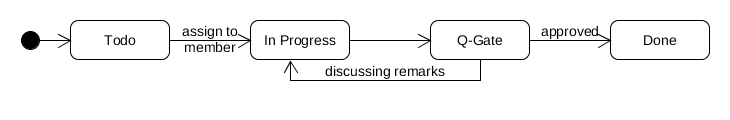
\includegraphics[width=0.9\textwidth]{images/state-quality.png}
        \caption{Quality Process}
        \label{fig:quality_process}
    \end{center}
\end{figure}

To ensure complete quality testing on the software every completed part will be assigned to a quality testing state. A team member that has not been part of the creation of the relevant piece then performs the quality testing.

\subsection{Requirements Quality Check}
\label{ssec:requirements_quality_check}

TODO Marco

\subsection{Deployment \& Manual Testing}
\label{ssec:deployment_manual_testing}

TODO Marco

\subsection{Testing \textit{React Native}}
\label{ssec:testing_react_native}

Like any software product, \textit{React Native} applications have to be tested for proper functionality and stability. As mentioned in \textit{\ref{ssec:deployment_manual_testing} \nameref{ssec:deployment_manual_testing}}, testing in this project was mainly done by simulating use cases and testing new functionality by hand, inputting values and user interaction into a deployed version of the application.
\newline
The manual testing approach was mostly taken since the existing base of the application proved to be largely incompatible. \textit{Appendix \ref{appendix:research_paper_sebastian_wilczek}: \nameref{appendix:research_paper_sebastian_wilczek}} contains a research paper detailing different testing frameworks and environments for \textit{React Native}, including usage examples and descriptions as to why they are incompatible or hard to use with the application in question.
\newline
Theoretically though, if the application did not show as many problems with existing testing frameworks, testing could be made more efficient by writing automatic end-to-end tests. One framework that can be made use of to write such tests is \textit{Appium}. Listing \ref{lst:appium_test} shows a test written \textit{WebdriverIO} in combination with \textit{Appium} that tests the application.

\begin{lstlisting}[language=javascript, caption=\textit{Appium} end-to-end test, label=lst:appium_test]
const webdriverio = require("webdriverio");
const opts = {
  port: 4723,
  desiredCapabilities: {
    platformName: "Android",
    platformVersion: "9",
    deviceName: "Nexus 5X API 28 x86",
    app: "[...]/SoFa/android/app/build/outputs/apk/debug/app-debug.apk",
    automationName: "UiAutomator2"
  }
};
describe("Basic Android interactions", function() {
  let client;
  beforeEach(function() {
    client = webdriverio.remote(opts);
    return client.init().pause(15000);
  });
  afterEach(function() {
    return client.end();
  });
  it("should click a tab that opens more functionality", async function() {
    return client
      .waitForExist('~More', 5000)
      .element('~More')
      .click()
      .waitForExist("~Privacy", 5000)
      .getText("~Privacy", function(result) {
        assert.equal(result.value, "Privacy");
      });
  });
});
\end{lstlisting}

The test is constructed relatively simple. It is first defined on what platform the test is supposed to be ran. In this case, it is an \textit{Android} device with the identification "Nexus 5X API 28 x86", which is the emulator running on the development machine. Furthermore, a path is given to an "apk" file, which is the build file of the application itself, telling the test that this is the application to be tested.
\newline
The actual tests are defined afterwards. In this example, the driver, which is \textit{WebdriverIO}, is supposed to connect to the emulator before each test and to disconnect afterwards. The test itself waits for an element with the \textit{Accessibility Label} "More" to exists, clicks that element, waits for another one with the value "Privacy", and finally checks if that component has the text value "Privacy". This is a simple test to see if the main screen of the application can switch between tabs. This test fails due to incompatibility reasons. For further information see the research paper mentioned at the beginning of this section.
\newline
Single \textit{React Native} components can also be tested using \textit{Jest}, which creates snapshots of component rendering and compares them each time the tests are ran. If there is a change in the rendering, the change is marked and the developer can decide whether the change is intentional or an error. If it is intentional, the snapshot is overwritten so it can be used during the next test.
\newline
However, \textit{Jest} is also largely unusable during this project. The nature of \textit{Jest} makes it more applicable to unit tests. Furthermore, since most of the newly developed components are functional components, \textit{Jest} also is unable to create snapshots, which means that these components can only be tested if they are first wrapped in non-functional components. This is a lot of extra work for the developers and is ultimately not worth it.

%% CONCLUSION
\section{Conclusion}
\label{sec:Conclusion}
\lhead{Conclusion}

At the beginning of the project, there was a lot of information to learn and the team was quiet optimistic to manage the three epics that the client from \textit{Connected.Football} provided. The first eight weeks were mainly spend understanding the language and frameworks that are used and writing all the necessary documents. It was a great experience working with real customers besides studying everything theoretical at University. The customer was a patient customer who did take his time to help and explain basic concepts of the programming language and frameworks. With the help of \textit{Jira} and \textit{GitHub} a real working scenario came up so students could work the way it is properly done. In the project different roles had been assigned so that everybody had different roles and responsibilities to take care of. After the first eight weeks everybody was familiar with the tech stack and their role in the project.
\newline
After having a basic understanding of the technology the group started developing the features. While working on the first epic plenty of unforeseen problems occurred that required a vast majority of time to understand, debug and fix. Due to these issues a lot of valuable time for the development was lost and sprints were overdue. Problems accumulated and the group was stuck at certain points by trying to fix tough errors, e.g. \textit{NPM} updating packages in the background without everybody knowing and breaking the application.
\newline
Roughly a month before the end of the project the group realised that they are far from successfully finishing the project. Every distraction was removed and the main focus was polishing up the results and communicating failure with the customer. The customer was nice and the only thing he wished for was a well documented handover document so that a new group of students can pick up the code and expand it.
\newline
Even though one epic was successfully finished the group learned a lot about \textit{JavaScript}, functional programming, \textit{NPM}, Firebase and all the used frameworks like \textit{React}, \textit{React Native}, \textit{recompose} and \textit{GraphQL}. With this valuable knowledge the group is able to get into \textit{JavaScript} code faster and work themselves through \textit{React Native} applications.

%% CHEAT SHEET
\section{Cheat Sheet}
\label{sec:cheat_sheet}
\lhead{\thesection \space Cheat Sheet}

\subsection{Paragraphs}
\label{ssec:paragraphs}

You can divide paragraphs with new lines.
\newline
This way you can write multiple paragraphs.

\subsection{Text Formatting}
\label{ssec:formatting}

Text can be \textit{italic} or \textbf{bold}.

\subsection{Lists}
\label{ssec:lists}

\subsubsection{Enumerated Lists}
\label{sssec:enum_lists}

\begin{enumerate}
    \item A list
    \item with numbers
    \begin{enumerate}
        \item and subcharacters
    \end{enumerate}
\end{enumerate}

\subsubsection{Itemised Lists}
\label{sssec:item_lists}

\begin{itemize}
    \item A list
    \item with items
    \begin{itemize}
        \item and subitems
    \end{itemize}
\end{itemize}

\subsection{Figures}
\label{ssec:figures}

\begin{figure}[H]
    \begin{center}
        
\includegraphics[width=0.5\textwidth]{images/figure.jpg}
        \caption{An included figure}
        \label{fig:figure}
    \end{center}
\end{figure}

\subsection{Tables}
\label{ssec:tables}

\begin{table}[H]
    \centering
    \begin{tabular}{|l|l|l|}
        \hline
            Title   & Title   & Title   \\ \hline
            Content & Content & Content \\ \hline
            Content & Content & Content \\ \hline
    \end{tabular}
    \caption{Some Table}
    \label{tab:some_table}
\end{table}

\subsection{References}
\label{ssec:references}

You can reference a chapter by number and name: \ref{sssec:item_lists} \nameref{sssec:item_lists}.
\newline
You can also do this for figures, tables, appendices and listings: \ref{fig:figure} \nameref{fig:figure}.

\subsection{Citation}
\label{ssec:citation}

You can cite any defined source from the file \textit{"bibliography.bib"} (\cite{google}).
\newline
".. some [...] citation [sic]." (\cite{some-master}).
\newline
Citations can be appended with further details. (\cite[p. 169]{my-book})

\subsection{Listings}
\label{ssec:listings}

\begin{lstlisting}[language=javascript,caption=Some JavaScript Code,label=lst:code]
describe("Hello", function() {
  //A comment
  someFunction("I run JavaScript", async function() {
    return true;
  });
});
\end{lstlisting}

%% BIBLIOGRAPHY
\newpage
\addcontentsline{toc}{section}{List of References}
\lhead{List of References}
\printbibliography{}

%% APPENDIX
\newpage
\lhead{Appendices}
\patchcmd{\appendices}{\quad}{: }{}{}
\begin{appendices}

\section{Research Paper Lucas Gehlen: TODO Add Title}
\label{appendix:research_paper_lucas_gehlen}

The following pages contain the research paper \textit{"TODO Add Title"}, written by the co-author Lucas Gehlen. It details TODO Add Summary.

%% TODO Add PDF
%% \includepdf[pages=-]{additional/research_report_lucas_gehlen_title} 

\newpage

\section{Research Paper Marco Kull: TODO Add Title}
\label{appendix:research_paper_marco_kull}

The following pages contain the research paper \textit{"TODO Add Title"}, written by the co-author Marco Kull. It details TODO Add Summary.

%% TODO Add PDF
%% \includepdf[pages=-]{additional/research_report_marco_kull_title} 

\newpage

\section{Research Paper Patrick Richter: TODO Add Title}
\label{appendix:research_paper_patrick_richter}

The following pages contain the research paper \textit{"TODO Add Title"}, written by the co-author Patrick Richter. It details TODO Add Summary.

%% TODO Add PDF
%% \includepdf[pages=-]{additional/research_report_patrick_richter_title} 

\newpage

\section{Research Paper Sebastian Wilczek: End-To-End Testing for React Native Applications}
\label{appendix:research_paper_sebastian_wilczek}

The following pages contain the research paper \textit{"End-To-End Testing for React Native Applications"}, written by the co-author Sebastian Wilczek. It details different frameworks that can be used to end-to-end test \textit{React Native} applications, both in general context as well as in the context of the \textit{Connected.Football} application.


\includepdf[pages=-]{additional/research_report_sebastian_wilczek_end_to_end_testing_for_react_native_applications}

\end{appendices}

\end{document}